\documentclass{beamer}
\usepackage{amsmath}
\usepackage{gvv}

\title{Question 4.13.5}
\author{AI25BTECH11040 - Vivaan Parashar}
\date{\today}

\begin{document}

\frame{\titlepage}

\begin{frame}
    \frametitle{Question: }
    The set of lines $ax + by + c = 0$, where $3a + 2b + 4c = 0$ are concurrent at the point \underline{\hspace{2cm}}.
\end{frame}

\begin{frame}
    \frametitle{Solution: }
    We are given the fact that $3a + 2b + 4c = 0$. This can be written as:
    \begin{align}
        \implies \myvec{3 & 2 & 4} \myvec{a \\ b \\ c} = 0 \label{eq1}
    \end{align}
    Let the point of concurrency be $\vec{P}$, at coordinates $\myvec{p_x \\ p_y}$. Because $\vec{P}$ lies on all lines $ax + by + c = 0$, we can write the following system of equations:
    \begin{align}
        \myvec{3 & 2 & 4 \\ p_x & p_y & 1} \myvec{a \\ b \\ c} = \myvec{0 \\ 0} \label{eq2}
    \end{align}
\end{frame}
\begin{frame}
    For this system to have a non-trivial solution in $a$, $b$ and $c$, and for the two original equations to be linearly dependent (since equation \ref{eq2} should be true whenever \ref{eq1} is true), the rank of the coefficient matrix must be 1.
    Applying row reduction:
    \begin{align}
        \myvec{3 & 2 & 4 \\ p_x & p_y & 1} &\xleftrightarrow{R_3 \rightarrow R_3 - \frac{R_1}{4}} \myvec{3 & 2 & 4 \\ p_x - \frac{3}{4} & p_y - \frac{1}{2} & 0}
    \end{align}
    Clearly, for the rank to be 1, the last row must be all zeros. Therefore the point of concurrency $\vec{P}$ is  $\myvec{\frac{3}{4} \\ \frac{1}{2}}$.
\end{frame}

\begin{frame}
    \frametitle{Plot: }
    \begin{figure}[h!]
        \centering
        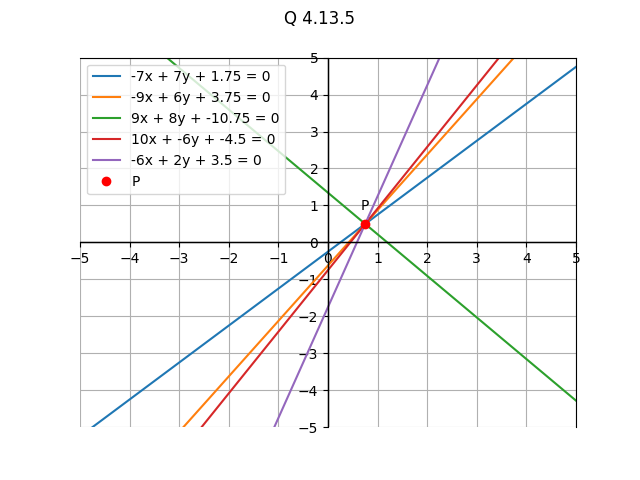
\includegraphics[width=0.8\columnwidth]{../figs/plot.png}
        \caption{Graph of lines with randomly generated values of $a$ and $b$ satisfying $3a + 2b + 4c = 0$. All lines are concurrent at the point $\myvec{\frac{3}{4} \\ \frac{1}{2}}$ (marked in red).}
        \label{fig:4.2.3}
    \end{figure}
\end{frame}

\end{document}
